%%%%%%%%%%%%%%%%%%%%%%%%%%%%%%%%%%%%%%%%%%%%%%%%%%%%%%%%%%%%%%%%%%%%
%% I, the copyright holder of this work, release this work into the
%% public domain. This applies worldwide. In some countries this may
%% not be legally possible; if so: I grant anyone the right to use
%% this work for any purpose, without any conditions, unless such
%% conditions are required by law.
%%%%%%%%%%%%%%%%%%%%%%%%%%%%%%%%%%%%%%%%%%%%%%%%%%%%%%%%%%%%%%%%%%%%

\documentclass{beamer}
\usetheme[faculty=science, university=uu, logo=temp-logo]{fibeamer}
\usepackage[utf8]{inputenc}
\usepackage[
	main=english
]{babel}
\title{Expanding on the Norwegian Linked Open Dataset} %% that will be typeset on the
\subtitle{Project Presentation} %% title page.
\author{Thomas Kaafjeld, Kent Odde and Stian Onarheim}
\usepackage{ragged2e}  % `\justifying` text
\usepackage{booktabs}  % Tables
\usepackage{tabularx}
\usepackage{tikz}      % Diagrams
\usetikzlibrary{calc, shapes, backgrounds}
\usepackage{amsmath, amssymb}
\usepackage{url}       % `\url`s
\usepackage{listings}  % Code listings
\frenchspacing
\begin{document}
\frame{\maketitle}

\AtBeginSection[]{% Print an outline at the beginning of sections
	\begin{frame}<beamer>
		\frametitle{Table of contents}
		\tableofcontents[currentsection]
	\end{frame}}

	\section{Introduction}

	\subsection{Linked Data}
	\begin{frame}{Linked Data}

		\begin{figure}
			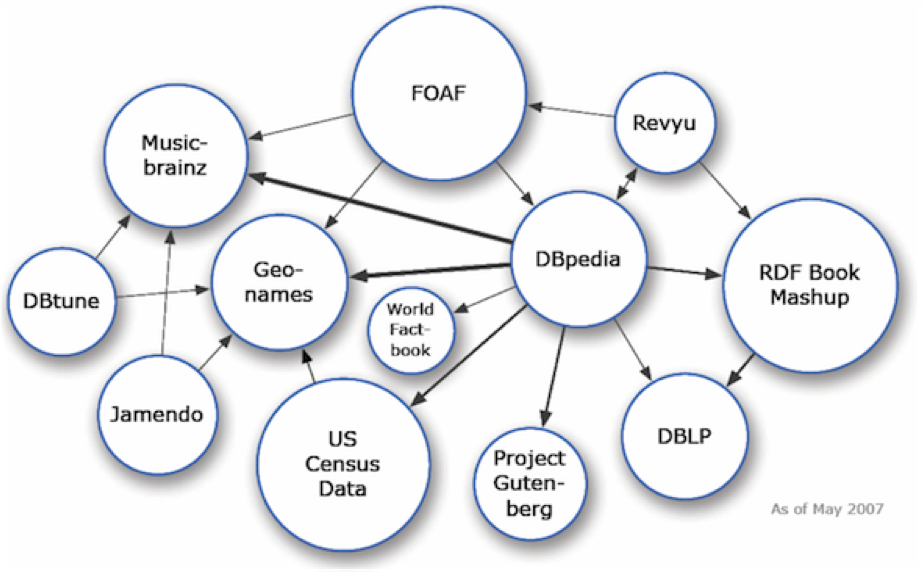
\includegraphics[scale=0.40]{resources/lod.png}
			\caption{A linked open data cloud\footnote[frame]{%
				Diagram taken from \url{linkeddata.center} }}
		\end{figure}
	\end{frame}

	\subsection{Norwegian Linked Open Data}
	\begin{frame}{Norwegian Linked Open Data}
		\begin{figure}
			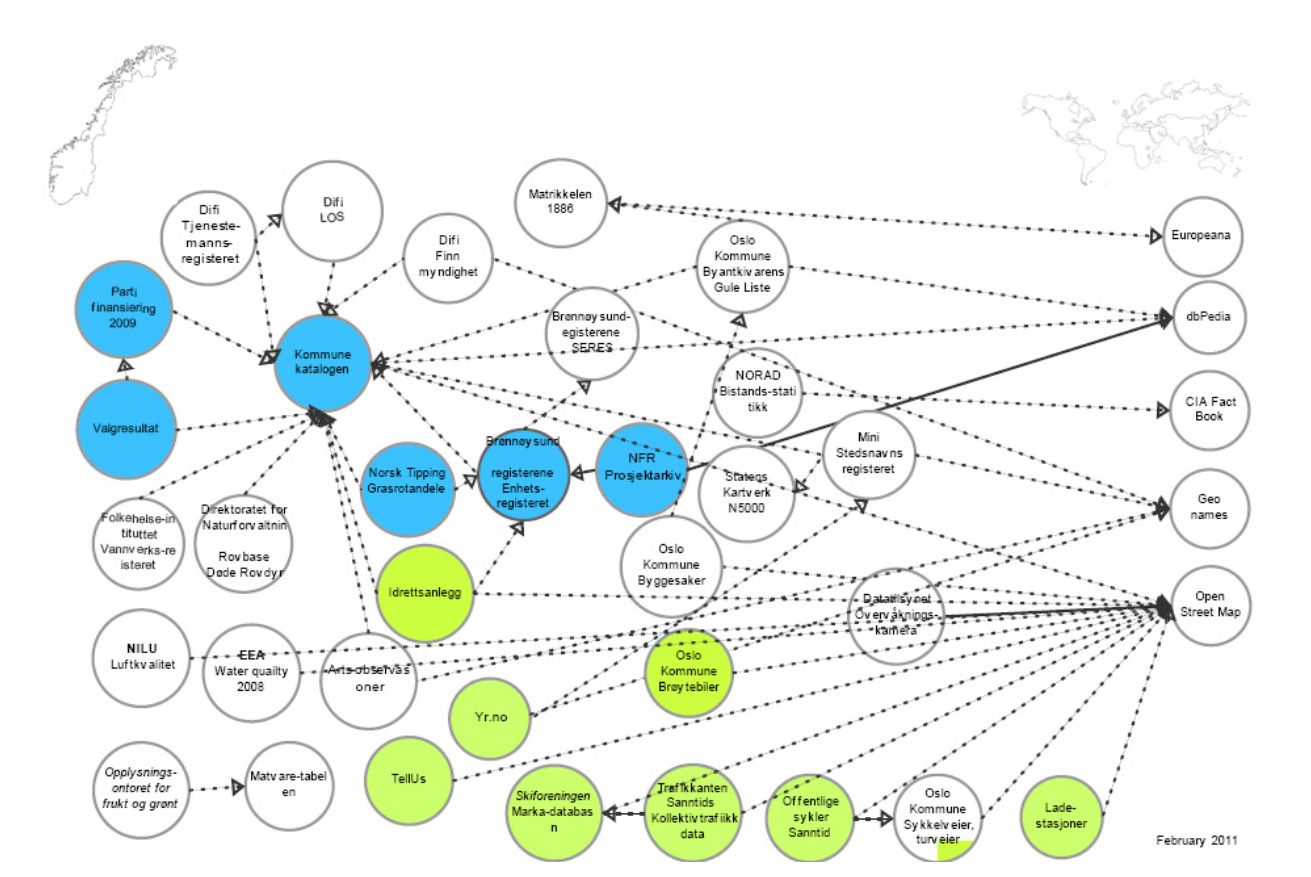
\includegraphics[scale=0.19]{resources/norwegian-lod.png}
			\caption{The Norwegian Linked Open Data\footnote[frame]{%
				Diagram taken from \url{semicolon.no} }}
		\end{figure}
	\end{frame}

	\subsection{Project Idea}
	\begin{frame}{Project Idea}
		\begin{itemize}
			\item Find norwegian open data that is not on the semantic web.
			\item Create an ontology.
			\item Link the data with existing linked open data.
			\item Publish it and get Tim Berners-Lee five stars.
		\end{itemize}
	\end{frame}

	\subsection{Data}
	\begin{frame}{Data}
		\begin{tikzpicture}[overlay,remember picture]
			\node[anchor=south east,xshift=-35pt,yshift=135pt]
			at (current page.south east) {
				
\includegraphics[width=35mm]{resources/sv.jpg}
				};
		\end{tikzpicture}%
		\begin{tikzpicture}[overlay,remember picture]
			\node[anchor=south east,xshift=-35pt,yshift=35pt]
			at (current page.south east) {
				
\includegraphics[width=35mm]{resources/posten.png}
				};
		\end{tikzpicture}%
		\begin{itemize}
			\item Parking data from Statens vegvesen\\
				(Norwegian Public Roads Administration).
			\item Provides data for 10638 parking facilities.
			\item Postal data from Posten\\
				(Norwegian postal service).
			\item Publicly available.
		\end{itemize}
	\end{frame}

	\section{Implementation}

	\subsection{Transforming \& Linking Data}
	\begin{frame}{Transforming \& Linking Data}
		\begin{figure}
			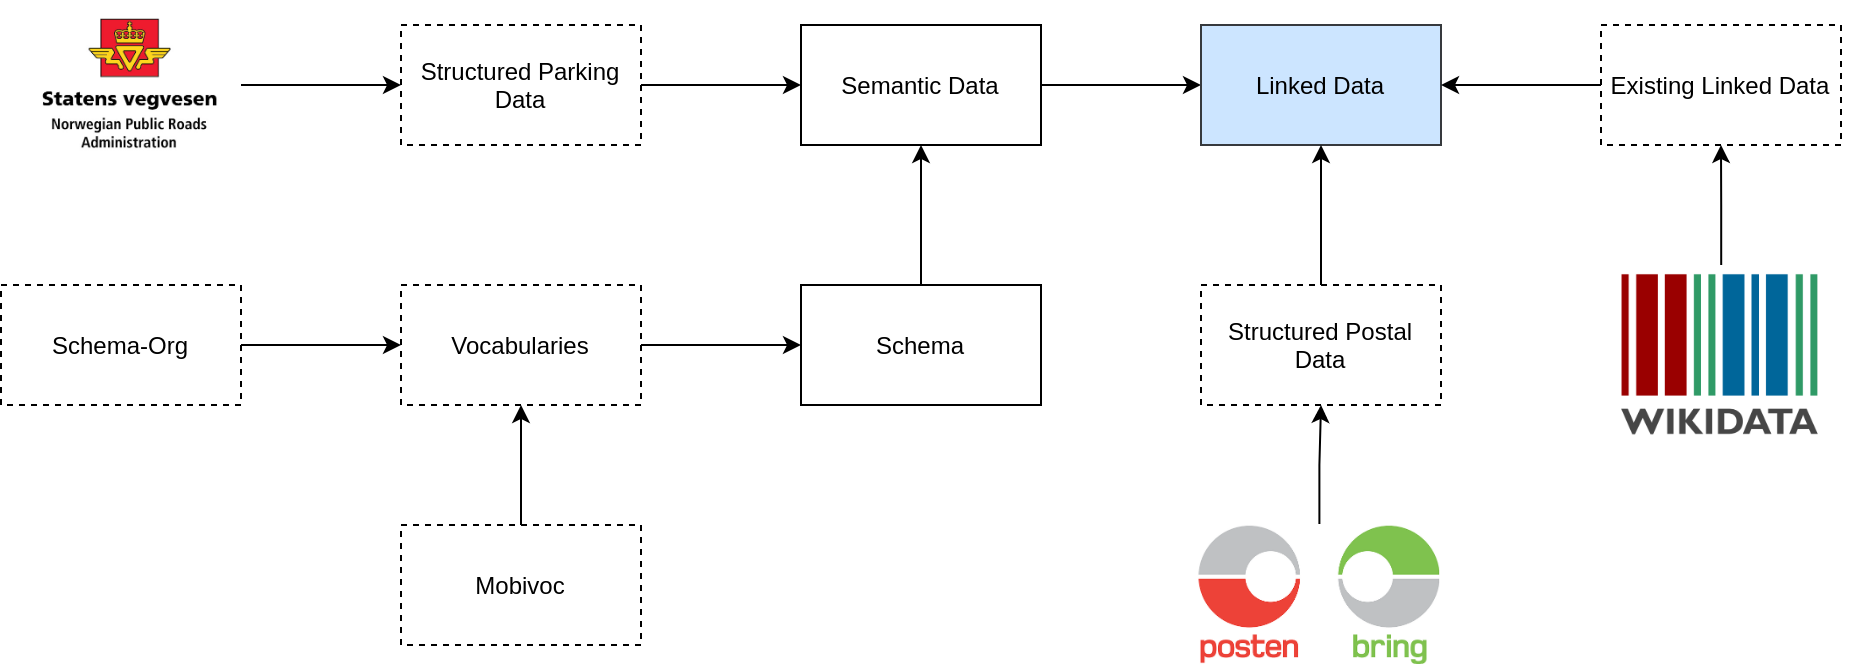
\includegraphics[scale=0.15]{resources/transform.png}
			\caption{Data Collection and Transformation}
		\end{figure}
	\end{frame}

	\subsection{The Ontology}
	\begin{frame}{The Ontology}
		\begin{figure}
			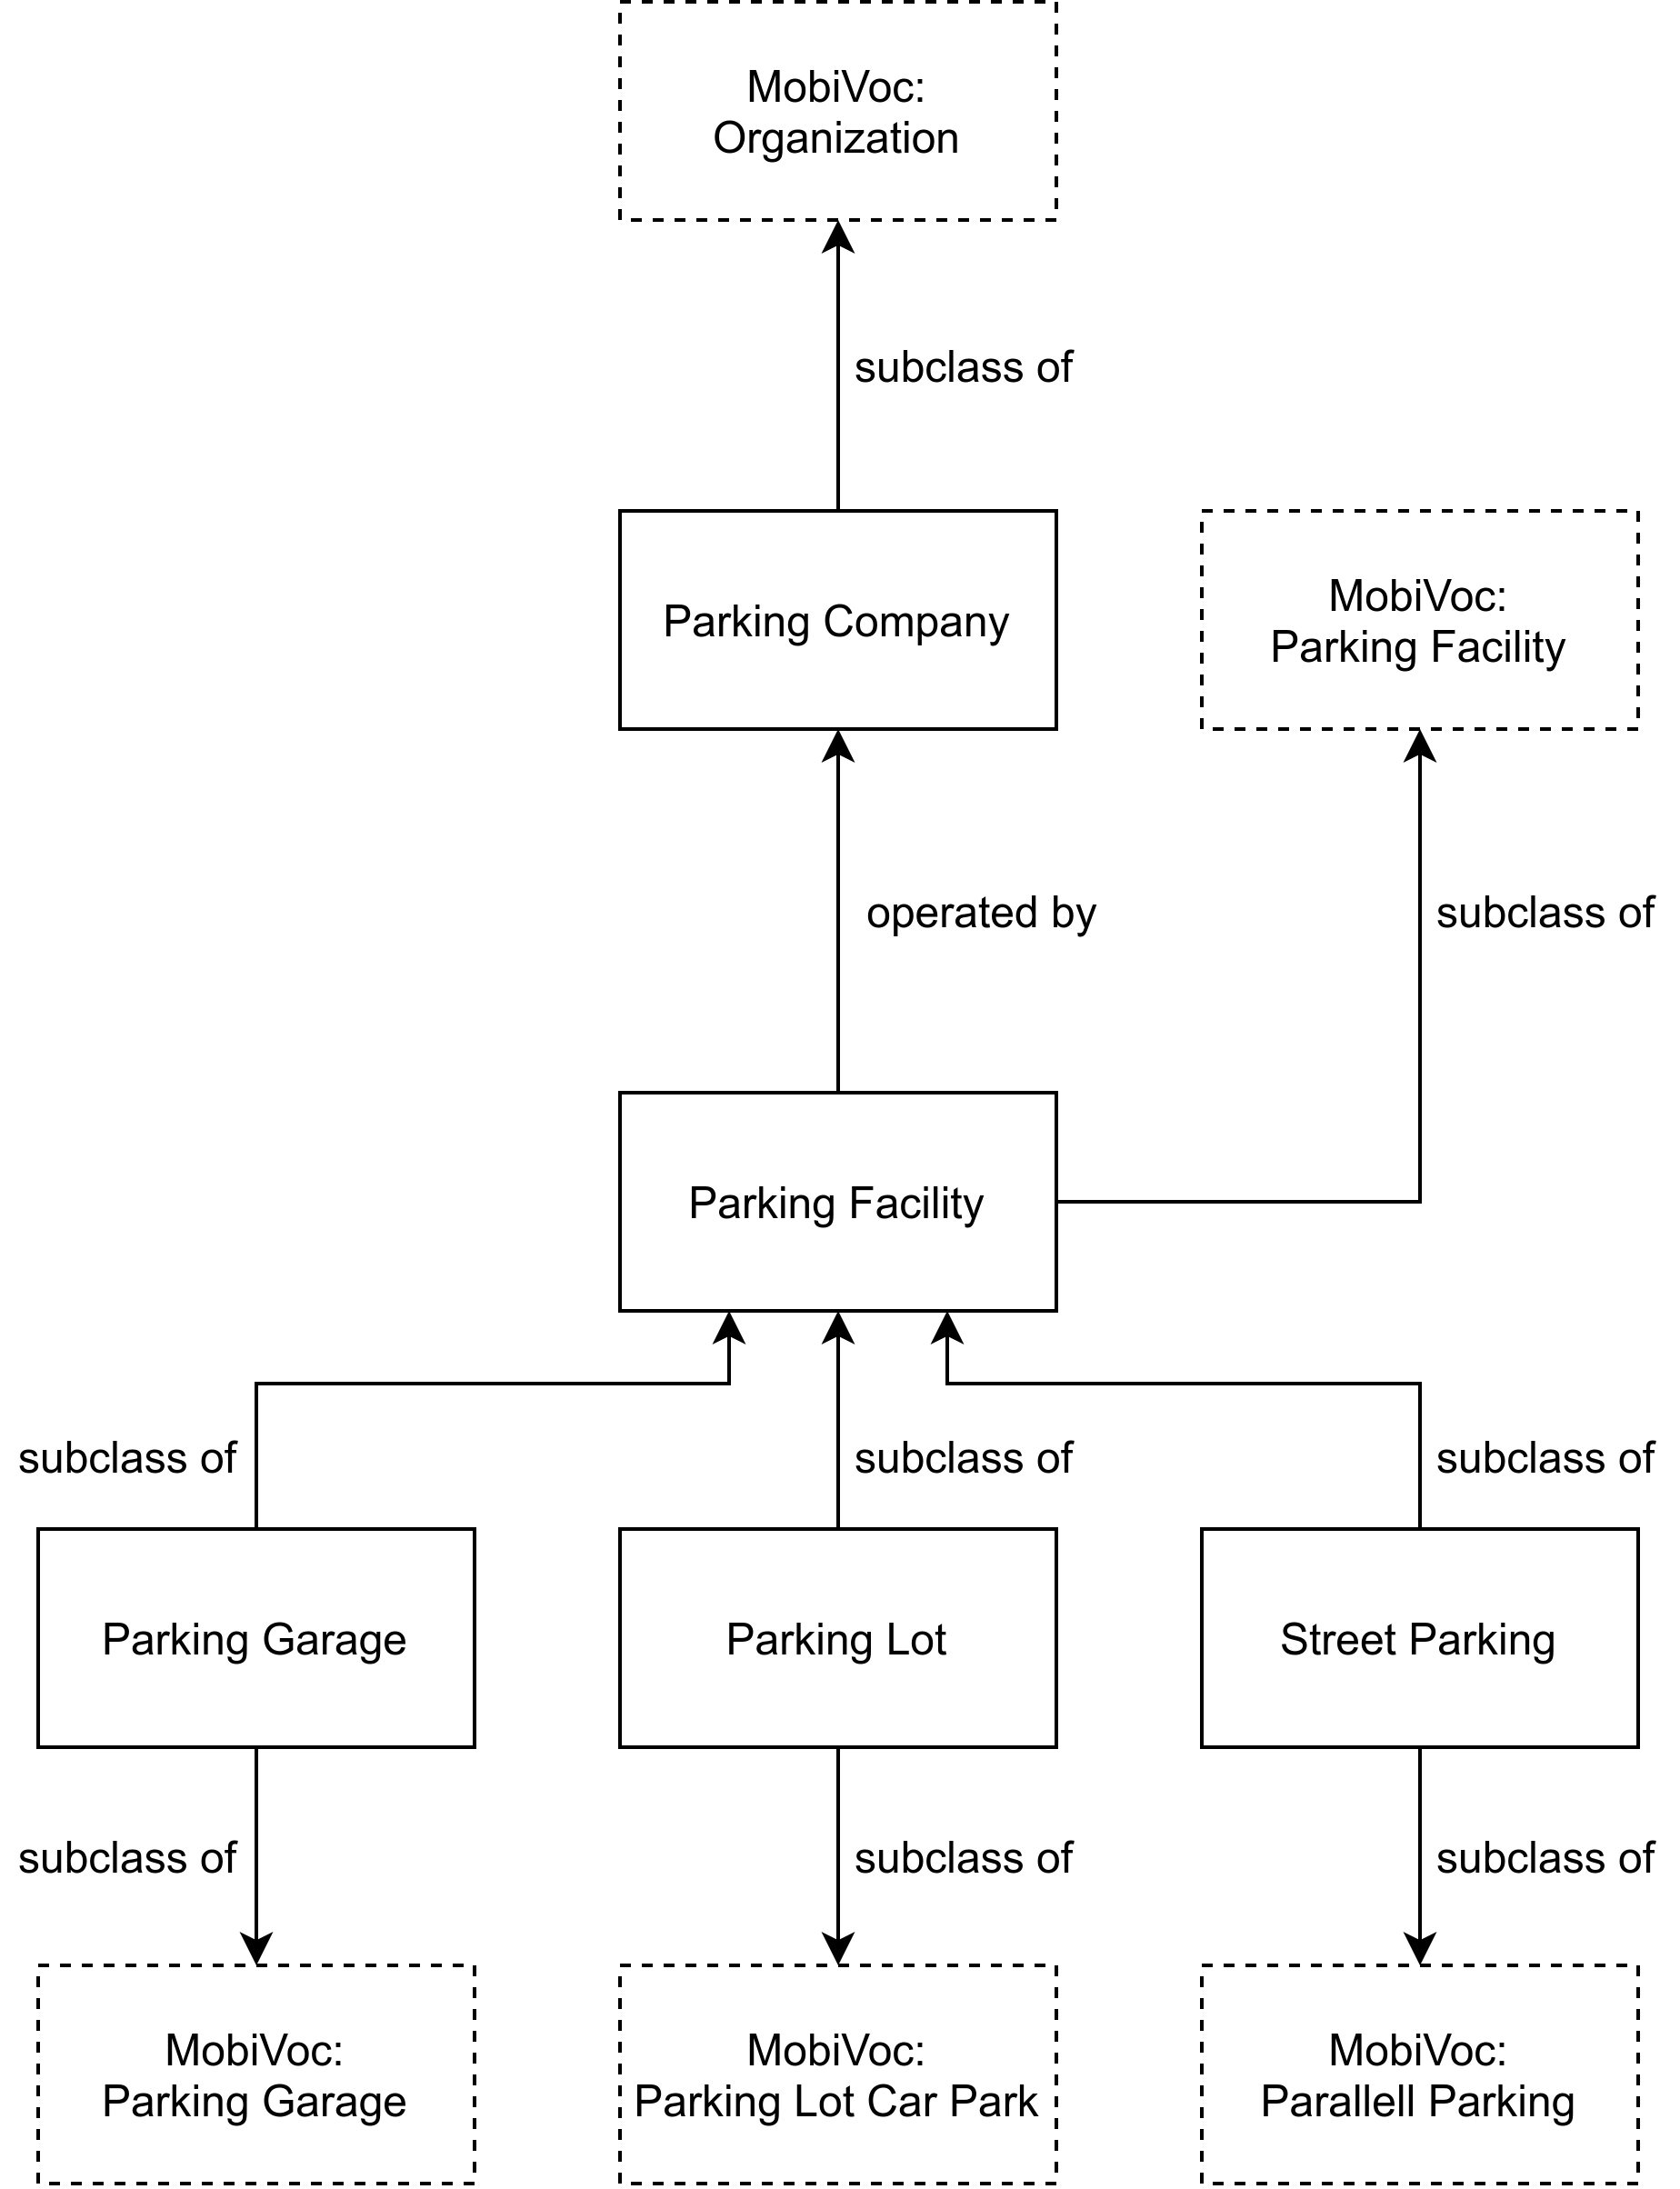
\includegraphics[scale=0.08]{resources/ontology-class.png}
			\caption{Classes}
		\end{figure}
	\end{frame}
	\begin{frame}{The Ontology}
		\begin{figure}
			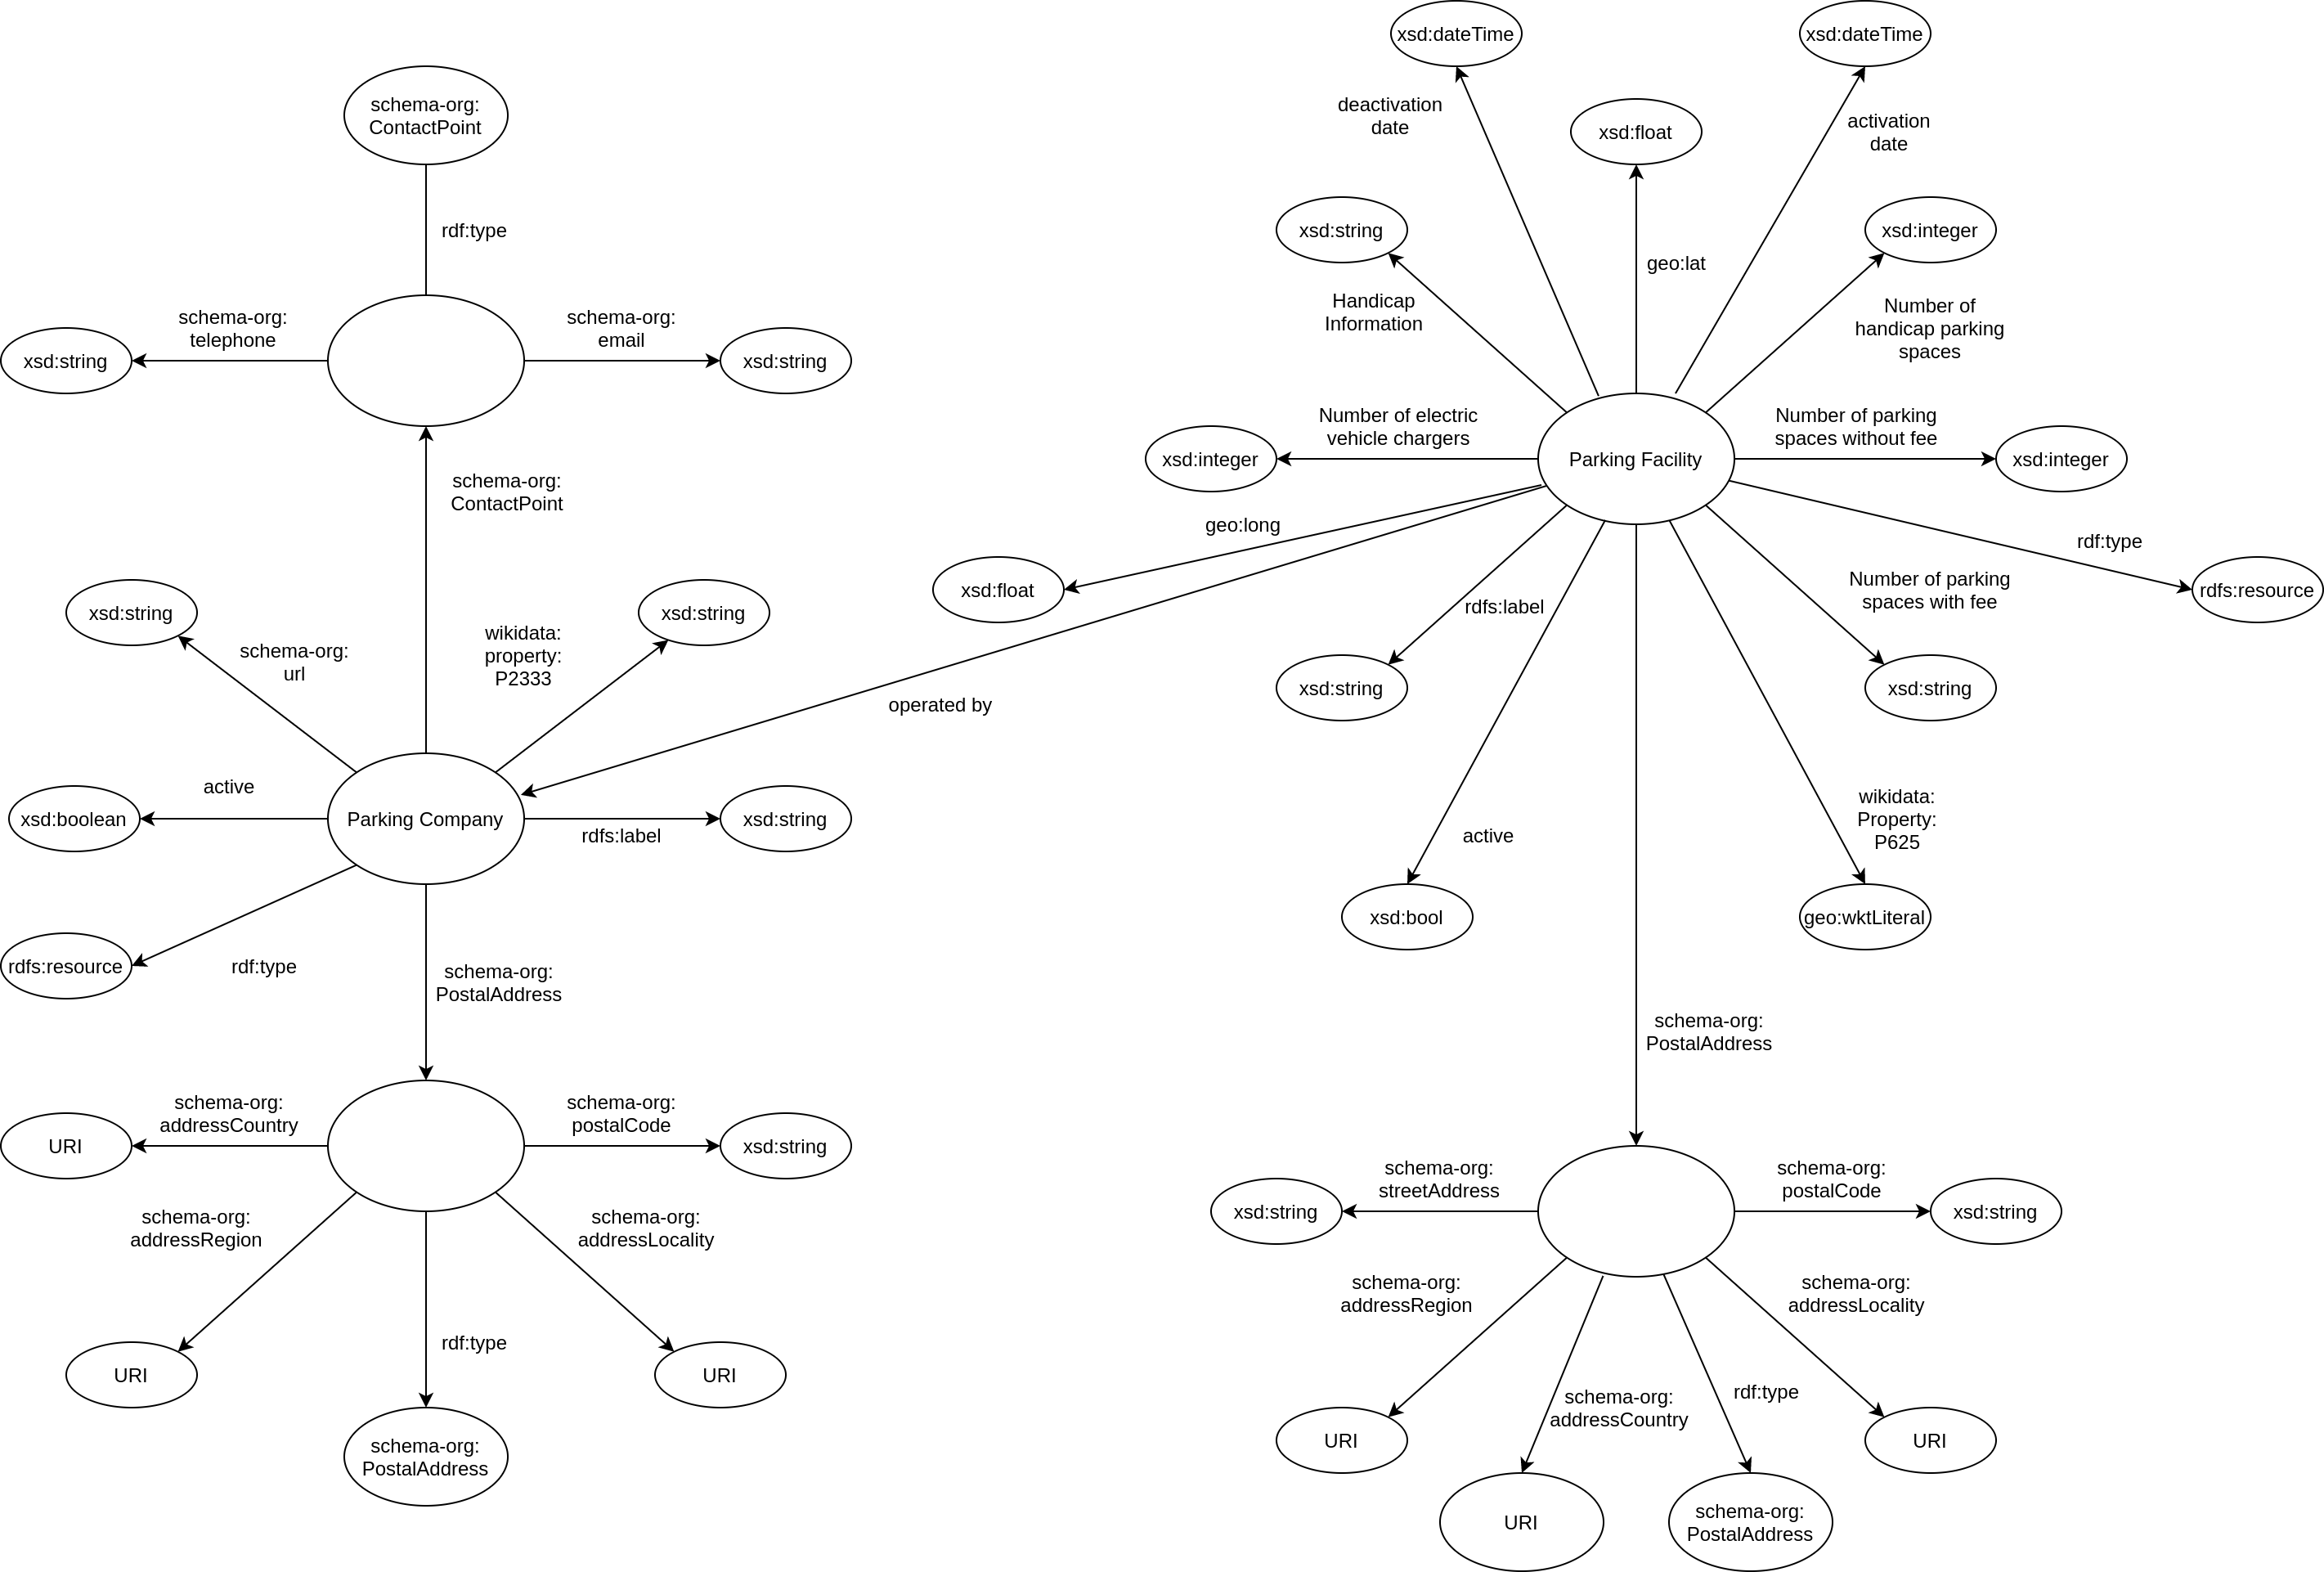
\includegraphics[scale=0.10]{resources/entities-attributes.png}
			\caption{Classes}
		\end{figure}
	\end{frame}
	\begin{frame}{The Ontology}
		\begin{figure}
			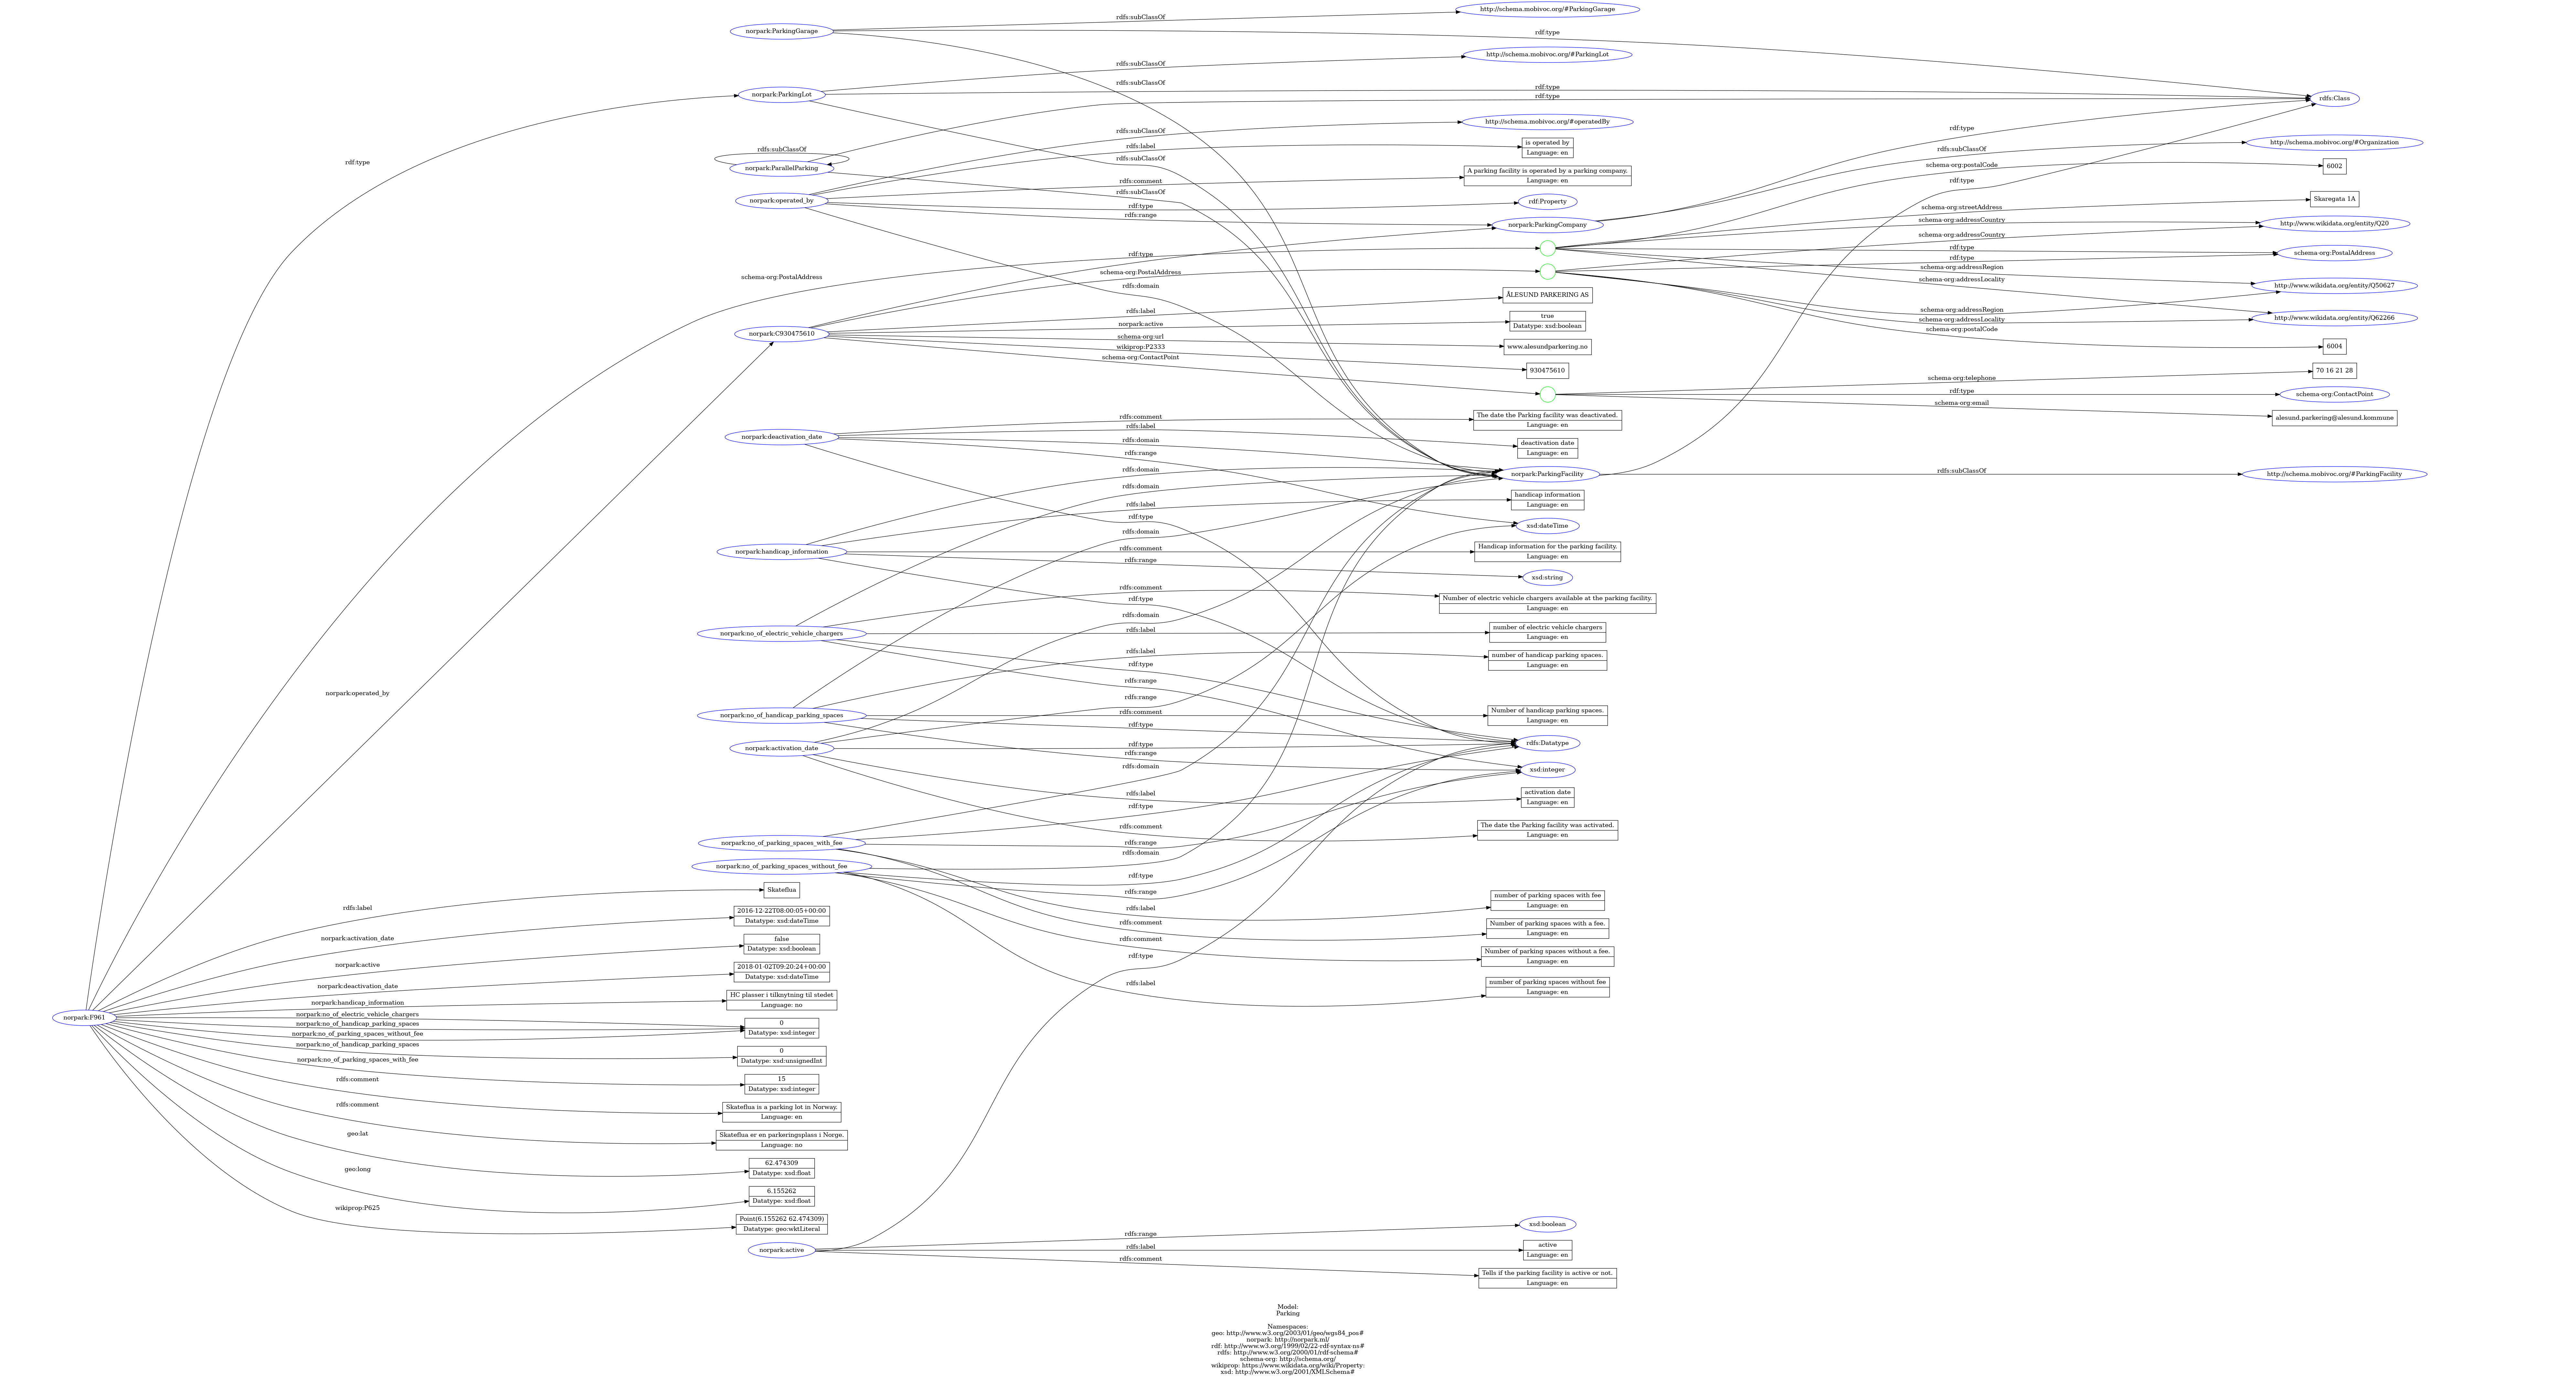
\includegraphics[scale=0.04]{resources/graph.png}
			\caption{Two Individuals}
		\end{figure}
	\end{frame}
	\subsection{System Architecture}
	\begin{frame}{System Architecture}
		\begin{figure}
			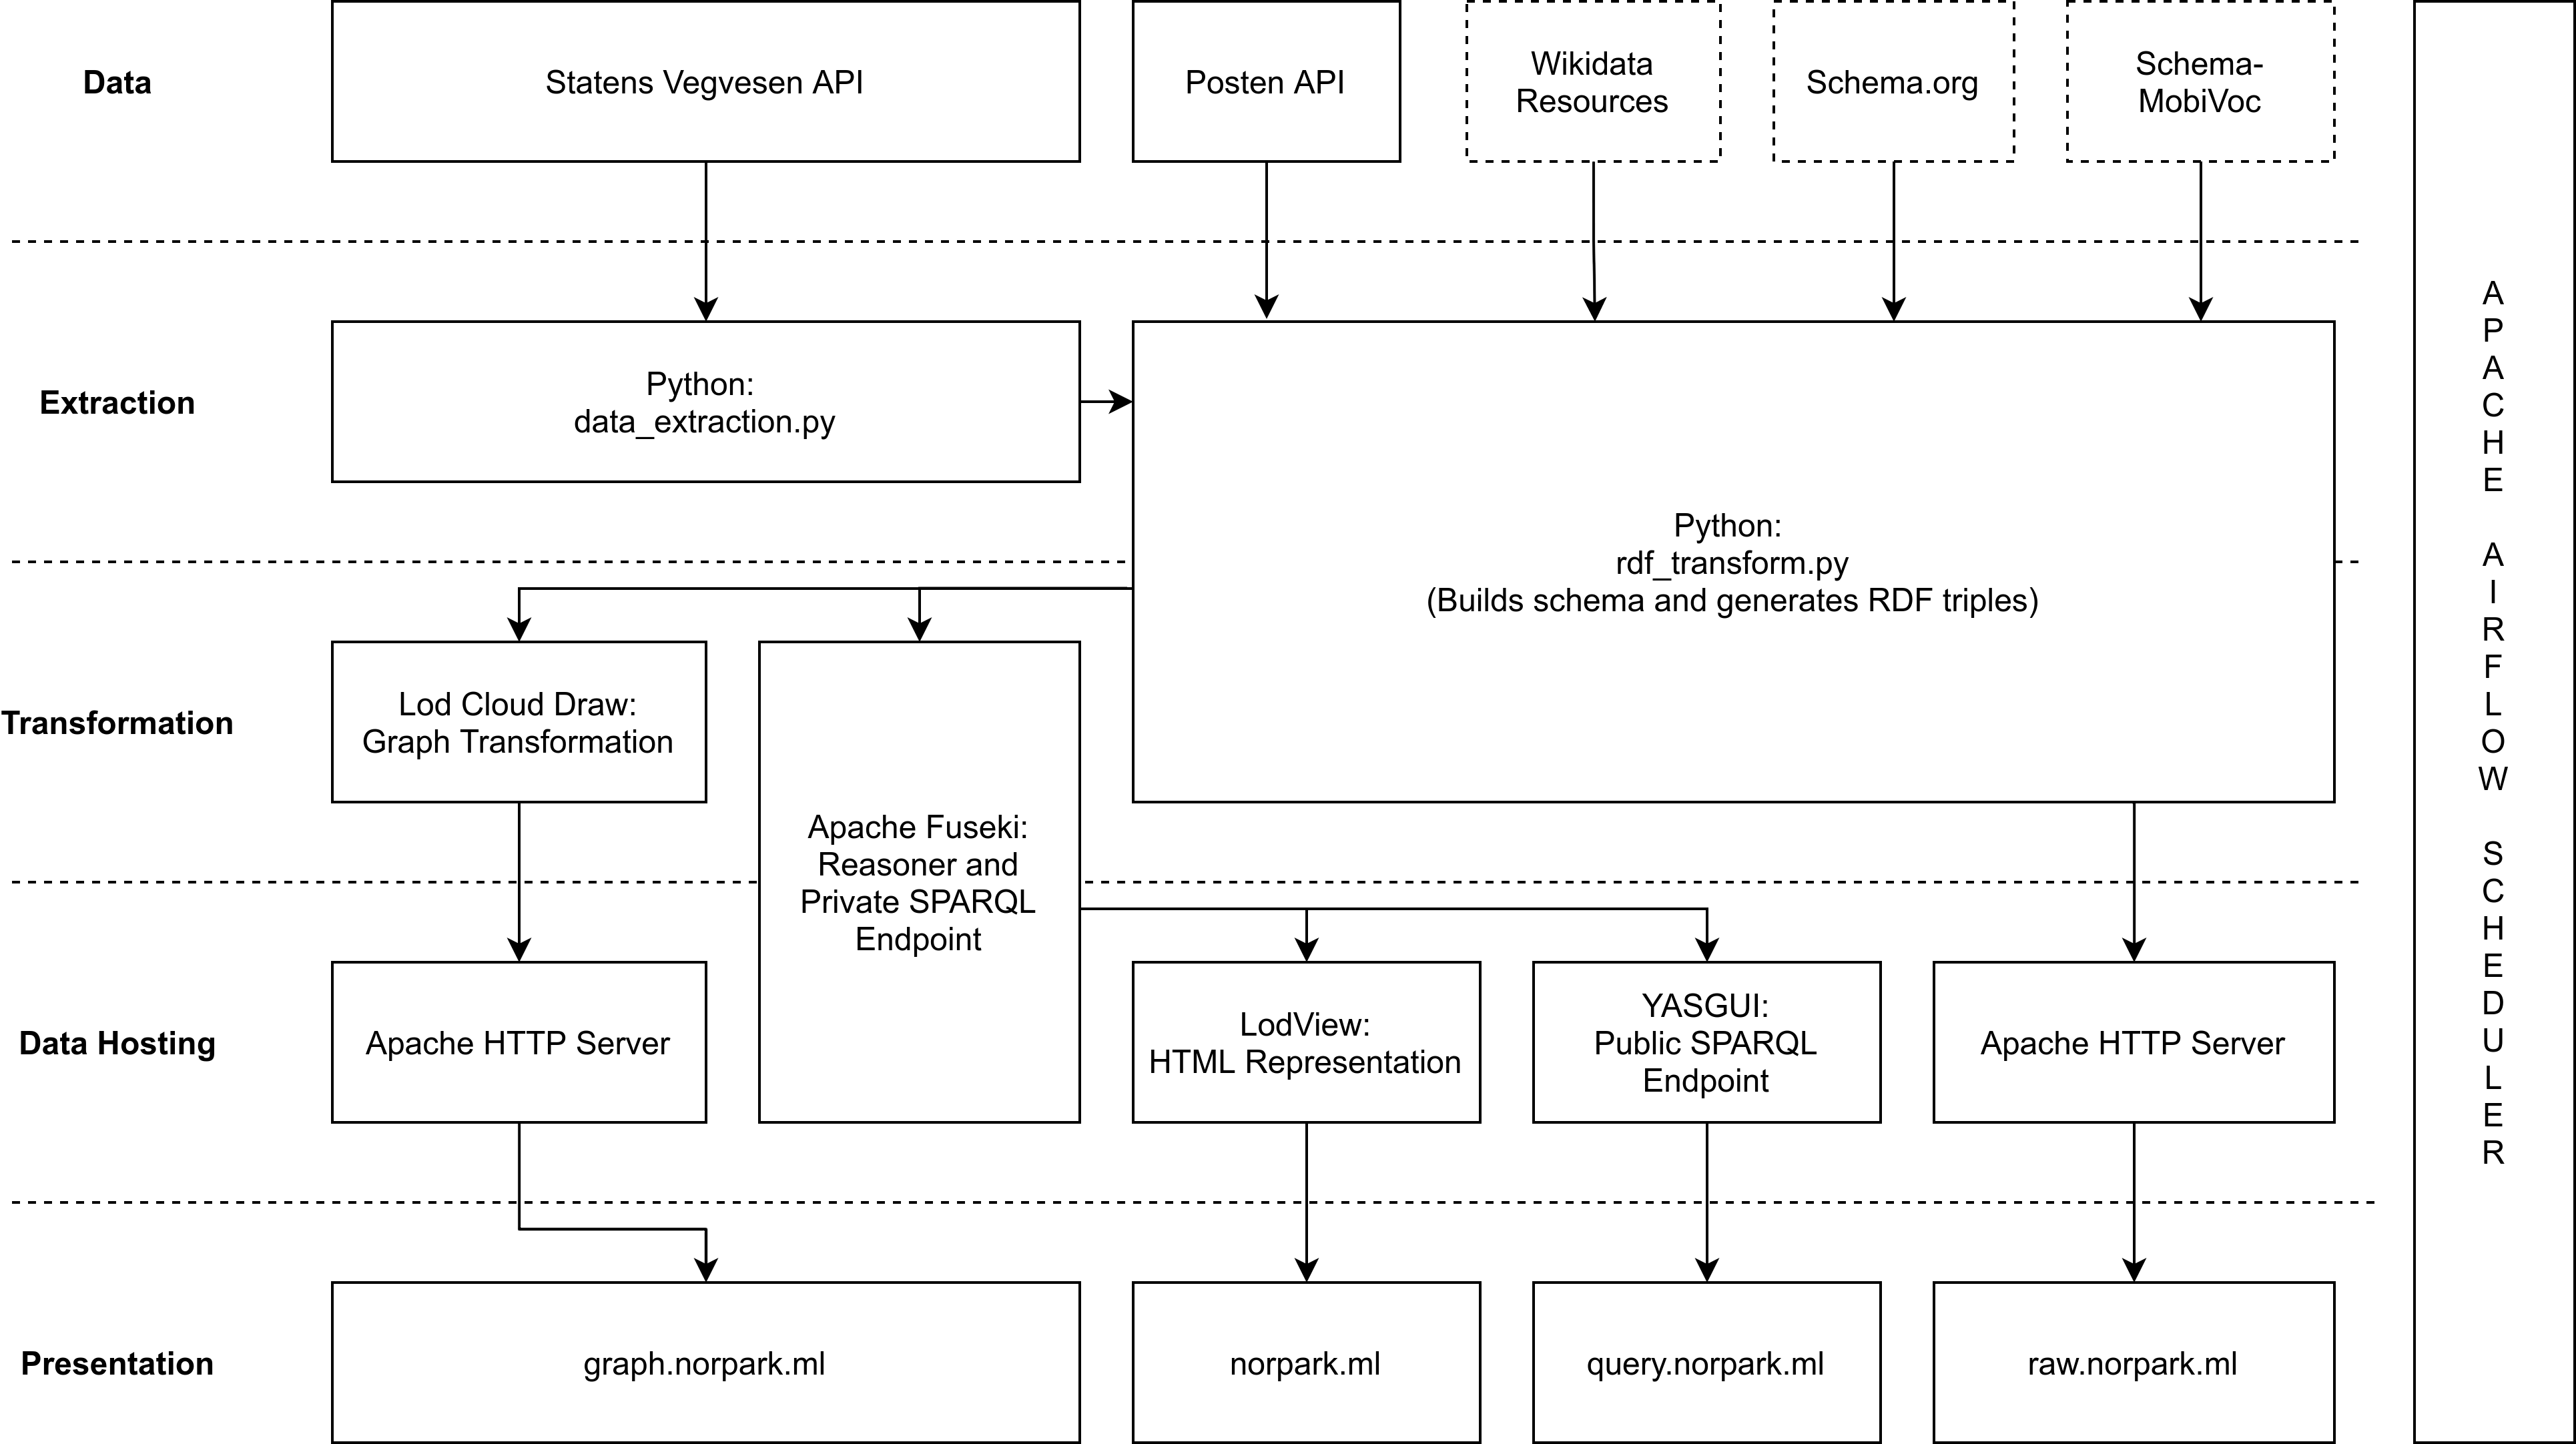
\includegraphics[scale=0.075]{resources/system-architecture.png}
			\caption{System Architecture}
		\end{figure}
	\end{frame}

	\section{Demonstration}
	\begin{frame}{Demonstration}
	\end{frame}

	\section{Conclusion}
	\begin{frame}{Conclusion}
		\begin{itemize}
			\item Added 244325 triples.
			\item Webpage
			\item Futureproof (Airflow).
			\item SPARQL endpoint.
		\end{itemize}
	\end{frame}

	\subsection{Five Stars}
	\begin{frame}{Five Stars}
		\centering
		\begin{tikzpicture}[remember picture,overlay]
			\node[xshift=-0cm,yshift=-2.2cm] at (current page.north){%
				
\includegraphics[scale=0.2]{resources/one-star.png}};
		\end{tikzpicture}
		Data is available on the Web, in whatever format.
		\vspace{26pt}
		\hrule
		\vspace{26pt}
		Our data is hosted publicly at http://norpark.ml
	\end{frame}

	\begin{frame}{Five Stars}
		\centering
		\begin{tikzpicture}[remember picture,overlay]
			\node[xshift=-0cm,yshift=-2.2cm] at (current page.north){%
				
\includegraphics[scale=0.2]{resources/two-star.png}};
		\end{tikzpicture}
		Available as machine-readable structured data, (i.e., not a scanned image).
		\vspace{26pt}
		\hrule
		\vspace{26pt}
		Our data is available in both .rdf and .ttl format, which are both machine-readable.
	\end{frame}

	\begin{frame}{Five Stars}
		\centering
		\begin{tikzpicture}[remember picture,overlay]
			\node[xshift=-0cm,yshift=-2.2cm] at (current page.north){%
				
\includegraphics[scale=0.2]{resources/three-star.png}};
		\end{tikzpicture}
		Available in a non-proprietary format, (i.e, CSV, not Microsoft Excel).
		\vspace{26pt}
		\hrule
		\vspace{26pt}
		Turtle and XML/RDF are both open-source.
	\end{frame}

	\begin{frame}{Five Stars}
		\centering
		\begin{tikzpicture}[remember picture,overlay]
			\node[xshift=-0cm,yshift=-2.2cm] at (current page.north){%
				
\includegraphics[scale=0.2]{resources/four-star.png}};
		\end{tikzpicture}

		Published using open standards from the W3C (RDF and SPARQL).
		\vspace{26pt}
		\hrule
		\vspace{26pt}
		Our data is in the form of RDF triples and can be queried with SPARQL.
	\end{frame}

	\begin{frame}{Five Stars}
		\centering
		\begin{tikzpicture}[remember picture,overlay]
			\node[xshift=-0cm,yshift=-2.2cm] at (current page.north){%
				
\includegraphics[scale=0.2]{resources/five-star.png}};
		\end{tikzpicture}

		All of the above and links to other Linked Open Data.
		\vspace{26pt}
		\hrule
		\vspace{26pt}
		Our data links to WikiData.org among others.
	\end{frame}

	\subsection{The Linked Open Data Cloud}
	\begin{frame}{The Linked Open Data Cloud}
		\begin{figure}
			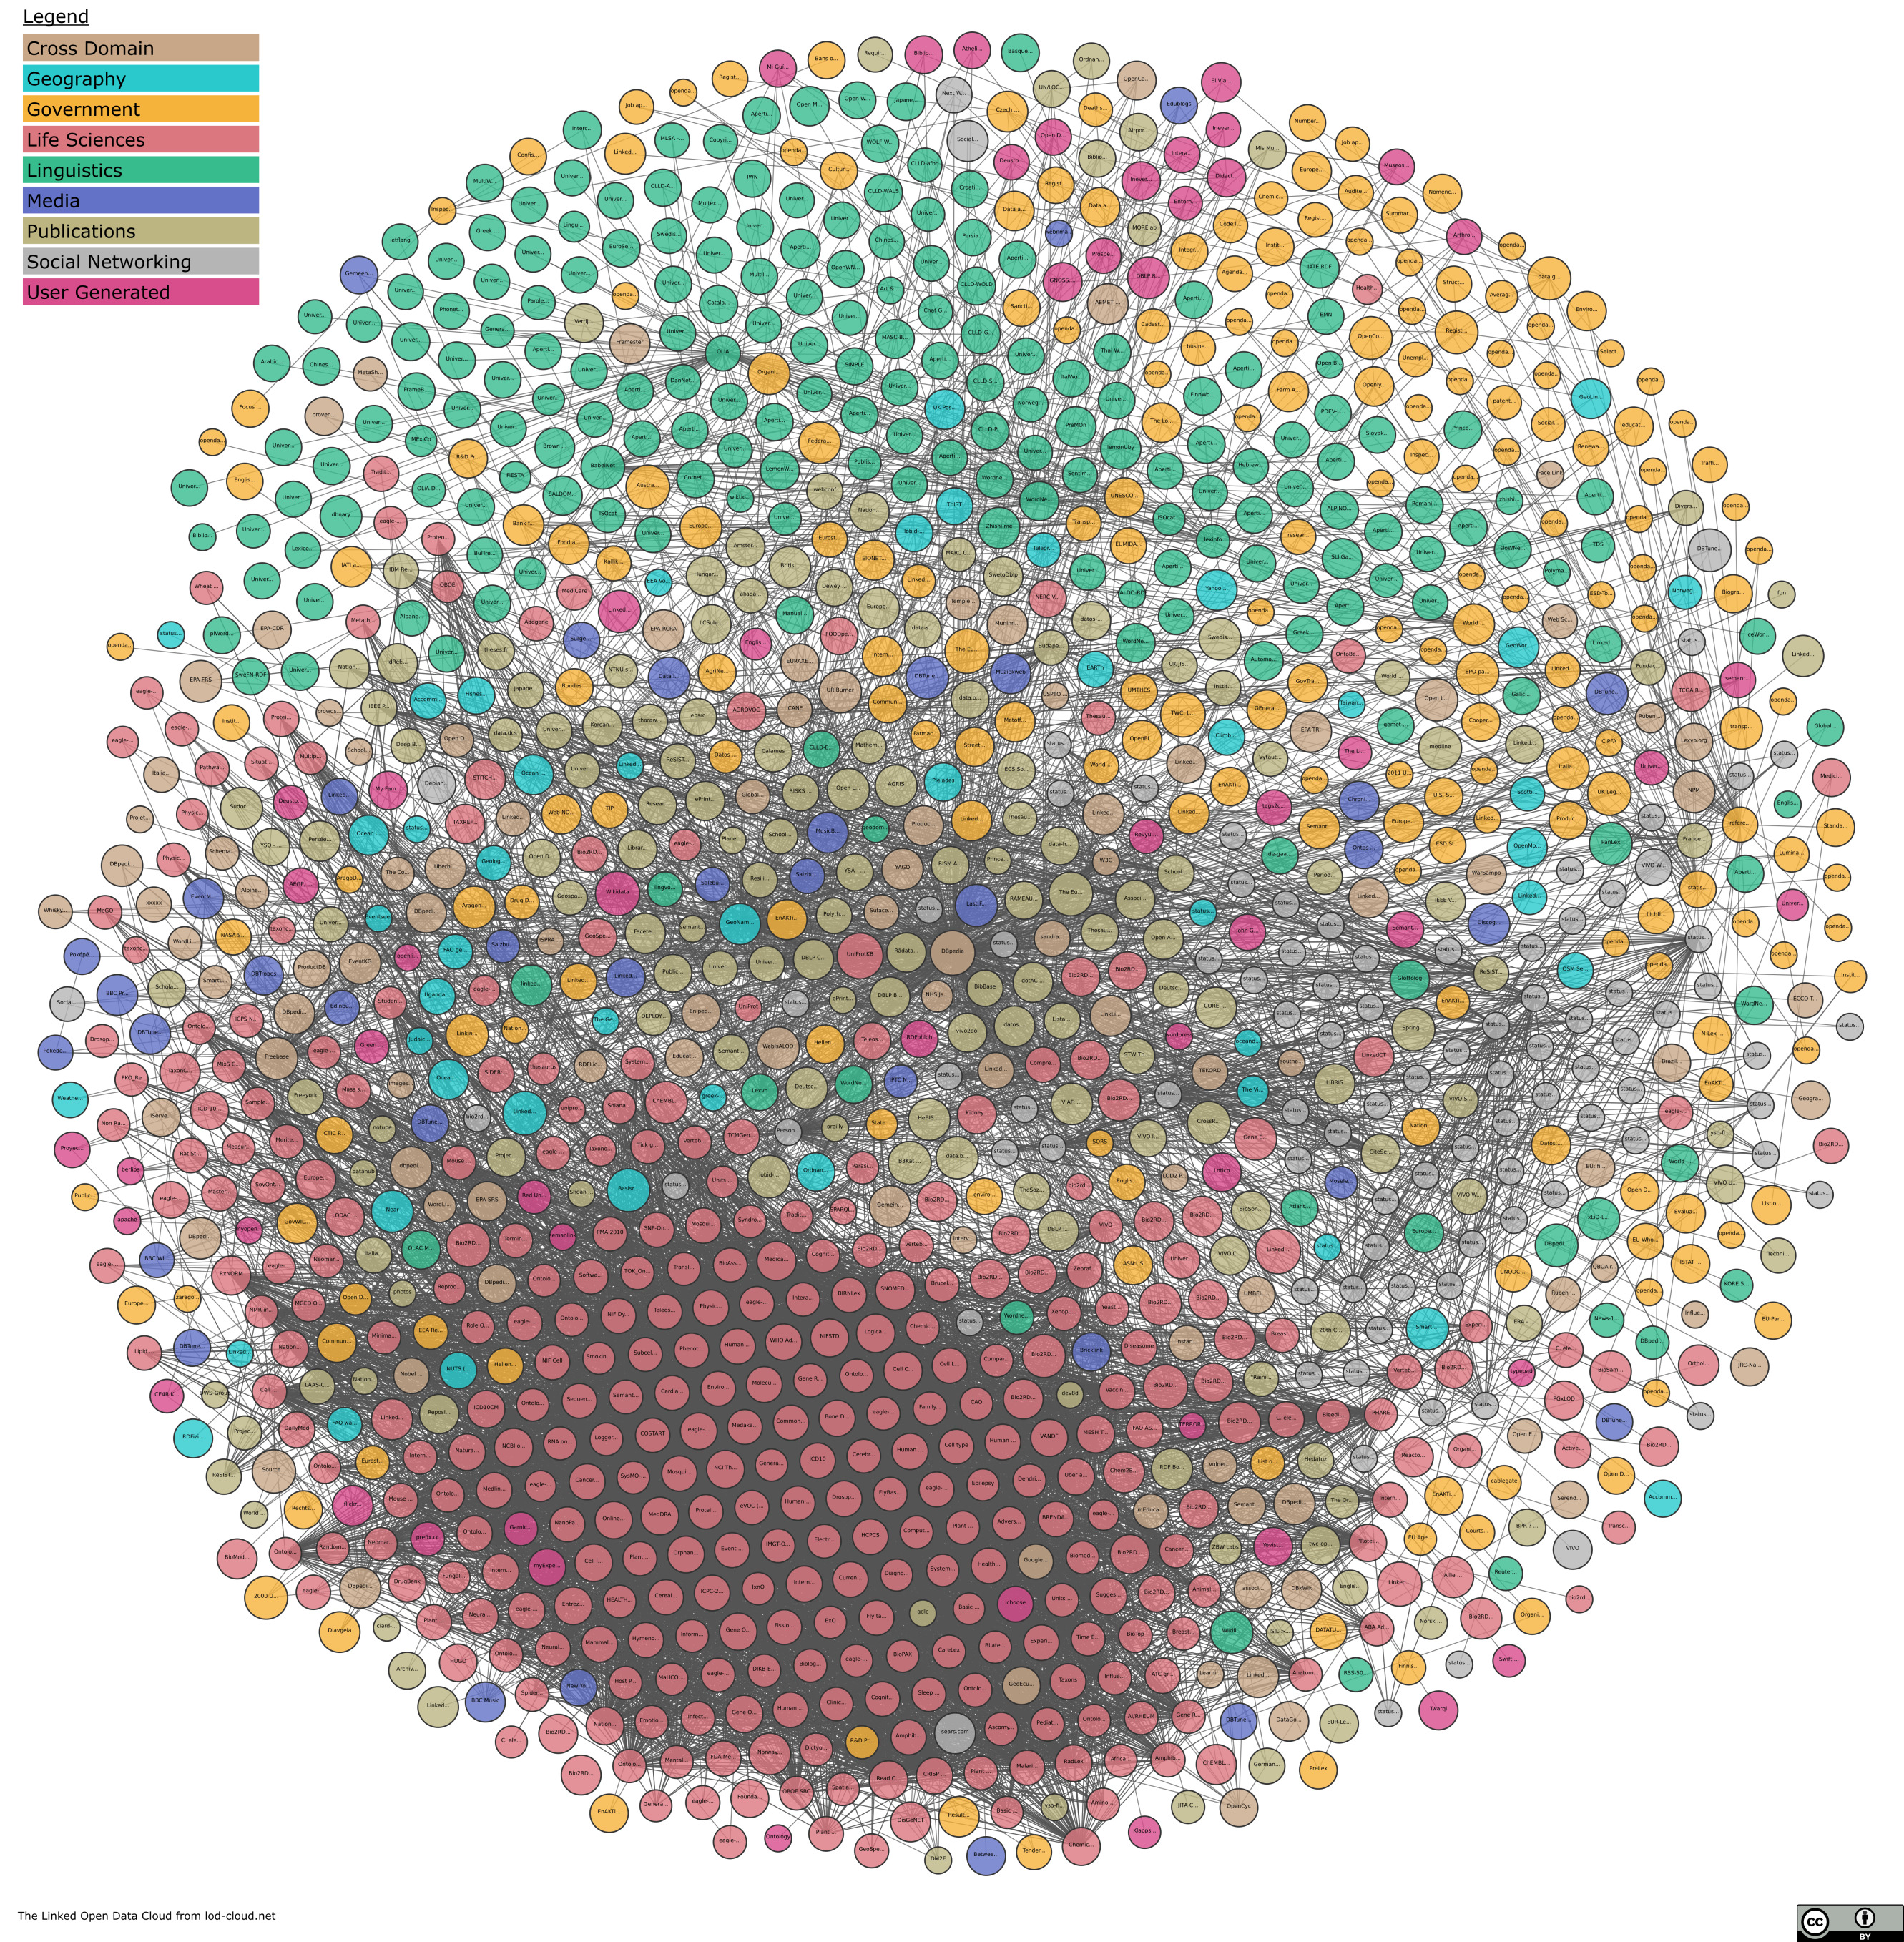
\includegraphics[scale=0.6]{resources/lod-cloud-sm.jpg}
			\caption{The Linked Open Data Cloud\footnote[frame]{%
				Diagram taken from \url{lod-cloud.net} }}
		\end{figure}
	\end{frame}

	\subsection{The semantic web today}
	\begin{frame}{The semantic web today}
		\begin{figure}
			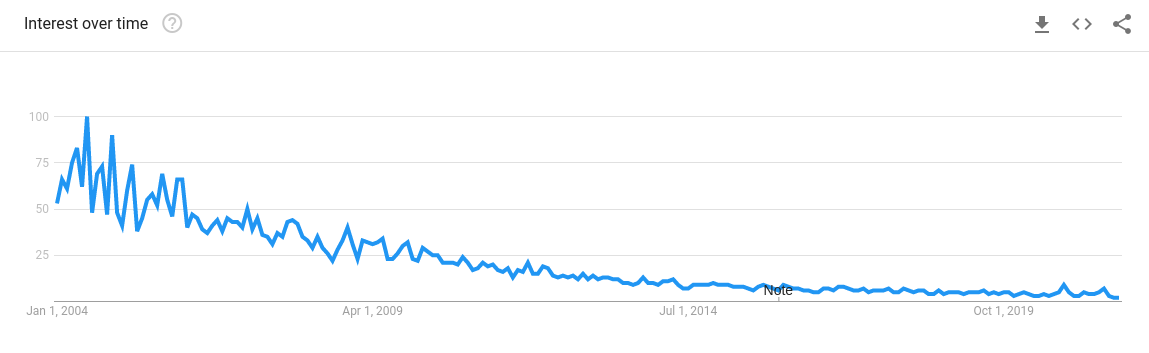
\includegraphics[scale=0.25]{resources/semantic-web-is-dead.png}
			\caption{Interest for the semantic web over time.\footnote[frame]{%
				Diagram taken from \url{trends.google.com} }}
		\end{figure}
	\end{frame}

	\subsection{Questions}
	\begin{frame}[label=questions]{Questions}
	\end{frame}


\end{document}
